\documentclass[FIPLY_base.tex]{subfiles}

%\author{Daniel Bersenkowitsch}

\begin{document}
\subsection{Promotion}
Es gibt dutzende Mittel um eine Android Applikation zu vermarkten. Ob über das Internet oder durch klassische physische Varianten lässt sich am Besten über Zielgruppenorientatierung bestimmen. 
[\citetitle{promteil1} \cite{promteil1}]

\subsubsection{Website}
Ein gute Methode um eine positive Reputation für seine Applikation zu schaffen ist es eine Website zu erstellen. Sie soll die Besucher einen kurzen Einblick in das Projekt und die Applikation bieten. Damit kann man bereits vor der Veröffentlichung eine positive Reputation schaffen und Benutzer von dem Projekt überzeugen, bevor das Produkt überhaupt auf dem Markt ist. Eine solche Teaser-Website sollte nur mit den minimalistischen Beschreibungen der Hauptfunktionen verkleidet werden, ein einfaches Design haben und einen guten Überblick über das Endprodukt aufzeigen: Als Beispiel Die Website der Applikation Instagram:

\begin{figure}[H]
	\centering
	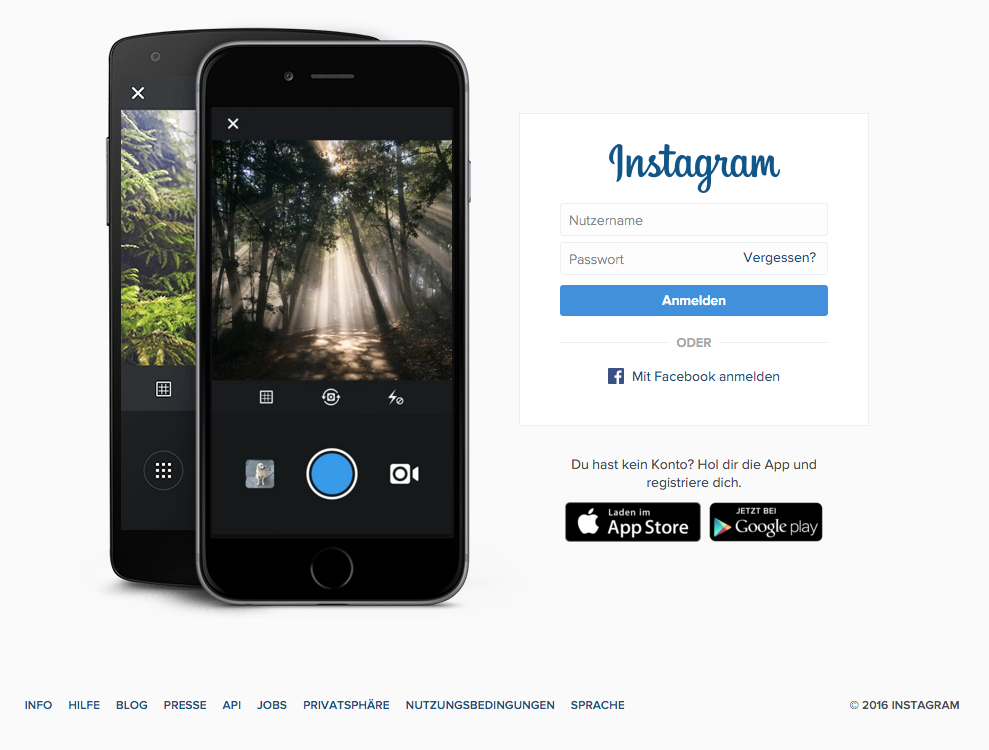
\includegraphics[scale=0.3]{img/instagramdotcom}
	\caption{Screenshot von http://instagram.com:}
\end{figure}
\ \\
Instagram.com ist ein gutes Beispiel für solch eine Teaser-Website. 
Eine weitere Möglichkeit ist es ein Video in die Website einzubauen, welche die Benutzung und Vorteile der Applikation aufzeigt. Eingebettet in die Seite kann dies durch verschiedene Videohoster wie: Youtube.com, Vimeo.com oder Vidme.com. Das Video in einem normales HTML5 Mediaplayer einzubetten ist auch ein beliebtes Mittel.

\subsubsection{Social Media Reputation}
Ein bereits seit langem wichtiges Element in der online Vermarktung ist die Social Media Reputation. Wenn man heutzutage seine Applikation an die Menschen bringen will, sollte das über die beliebten sozialen Netzwerke wie Facebook, Google+, Twitter, Instagram, Vine,... und unzähligen mehr passieren. Seiten wie diese bieten die Möglichkeit für das Produkt einen eigene Seite oder Account zu erstellen, über diesen sich dann Benutzer unterhalten und ausstauschen können und neue gewonnen werden können. Zusätzlich können Administratoren beliebter Facebook Seiten beispielsweise dafür bezahlt werden, damit sie die App darauf teilen und positive Merkmale dabei unterstreichen. 
\newline
Ein weiteres gutes Social Media mittel ist Reddit.com. Die Seite inkludiert die Funktion einen eigenen Developer Blog zu führen, worauf updates, bugs und neue Ideen für die Funktionalitäten der Applikationen geteilt werden können. Zusätzlich können bei dieser Webseite angemeldete User auch in diesem Blog posten - sich mit den Entwicklern unterhalten und mithelfen die App zu verbessern. Gute Vorschläge oder Ideen werden von Benutzern mit einem Pfeil nach oben markiert und wandern in der Postingliste hinauf damit die Sichtbarkeit steigt und sie mehr Personen lesen und darüber diskutieren können. Dies schafft eine sogenannte "Below-the-line"- Werbemöglichkeit für das Projekt.

\begin{figure}[H]
	\centering
	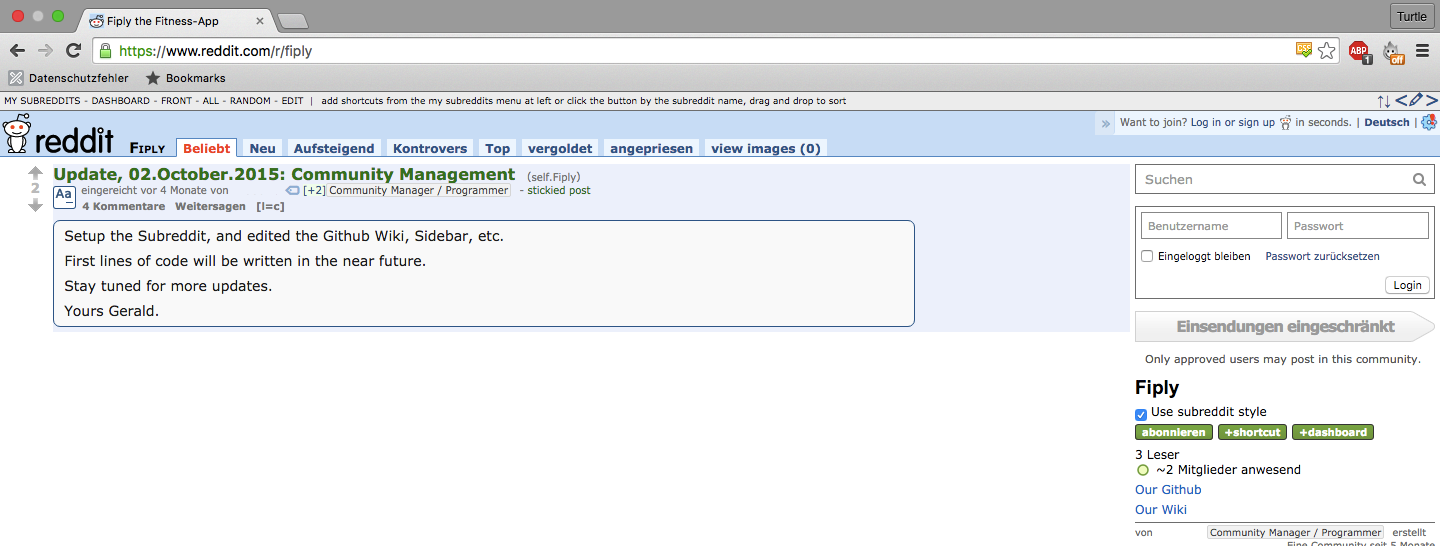
\includegraphics[scale=0.28]{img/fiplysubredditscreenshot}
	\caption{Screenshot von http://reddit.com/r/fiply}
\end{figure}

\subsubsection{Presse}
Eine der einfachsten Möglichkeiten ist es, eine Email an selektierte Schreiber die sich auf etwaige Bezugsthemen spezialisieren (Technik Blogs, Youtube- Review Kanäle oder wie bei dem Fiply Beispiel auch Fitnesstrainer/Fitnesscoaches und Fitnesscentern), auszusenden. Zu beachten ist dabei die persönliche Note. Jeder Aussendung sollte individuell zugeschnitten werden um den Empfänger anzusprechen. Inhalt soll knapp und bündig gehalten werden und die wichtigsten Informationen zusammenfassen wie zum Beispiel: die wichtigsten Funktionen, wichtige Links, Kontaktinformationen und Alleinstellungsmerkmale. Weiters ist zu überlegen, ob eventuelle kostenpflichtige Versionen dem Adressaten gratis übermittelt werden um ihn oder sie dafür zu motivern über das Projekt zu schreiben. 

\subsubsection{Wettbewerbe}
Kaum mit etwas anderem kann man schneller für Aufmerksamkeit sorgen als mit dem Gewinnen von Wettbewerben. Auch schon nur bei einer Einreichungen und Nominierung kann man einen hohen an Bekanntheitsgrad für seine App erlangen. Ein positiver Effekt ist auch, dass Gewinner und oft Zweit- und Drittplatzierte sich durch so eine Veranstaltung hin und wieder einen kleinen aber wichtigen Artikel in Zeitungen oder Onlinemagazinen, aber auch Technikblogs u.A. teilen. Wettberwerbe sind ein wichtiges Element um das Produkt an die Zielgruppen zu bringen. Am besten sieht man nach welche Art von Kategorien es bei Preisauschreiben gibt und reicht es dann dort mit der höchsten Gewinnchancen ein, oft kann man sein Projekt auch bei mehreren Kategorien gleichzeitig anmelden. 
\newline
Eventuelle Siege k"onnen auf der App-Homepage aufgeführt werden um Erstbesucher davon zu überzeugen, dass das geworbene Produkt Qualität aufweist.

\subsubsection{Persönliche Werbung}
In erster Linie sollte man seine Bekannten und Freunde um ein ehrliches Feeback bitten, ob das Projekt denn wirklich gut bei dem Endbenutzer ankommen kann. Objektive Meinungen von Freunden sind der Grundstein für die Erfolgsvorhersehung einer selbst erstellten Applikation. Die Verbreitung an Bekannte oder Verwandte kann durch persönliche Gespräche, Emails oder Social Media erfolgen. Am Besten bewährt sich dabei jedoch die persönliche Vermittlung. Mundpropaganda mag nicht sehr schnell sein, dafür aber sehr effektiv.

\subsubsection{Reklame}
Bei Reklamen/Werbeinschaltungen sollte in erster Linie auf die Zielgruppe geachtet werden. Erfolgreiche Reklame passiert nur durch zielgerichtete Zielgruppendefinition. Dabei sollte man sich Fragen stellen wie: Was will ich genau bewerben? Welche Personen will ansprechen? Durch welche Plattformen komme ich an diese Personen ran? Wie gestalte ich die Werbung möglichst attraktiv? \newline
Potentielle User kann man dort anwerben, wo sich diese aufhalten. Bei diversen Onlinecommunities in Foren, Websiten oder Applikationen mit verwandtem Inhalt oder Interessensgruppen. Dabei schränken sich die Möglichkeiten nicht nur auf physische Reklamemöglichkeiten wie Inserate oder Werbeplakate ein. Dienste wie Facebook, Twitter, Google Adsense bieten eine Umfangreiche Zielgruppenschaltung zu entsprechenden Preisen an. Aber auch auf Radio und Televisionswerbung muss nicht verzichtet werden.


\subsubsection{In Appstore Optimierung (IAO)}
Genau wie bei einer Suchmaschinenoptimierung für Webseiten bei Diensten wie Google.com gibt es dies auch für Applikation im Google Playstore. Ziel ist es, dass der potentielle Benutzer durch verschiedene, möglichst wenige, bestimmte Stichwörter in der Suchanfrage auf die Applikation stoßt. Mehr als 50\% der Nutzer einer App entdecken diese durch das erstmalige Suchanfrage bestimmter Stichwörter in dem Store.
\newline
Bei der Einrichtung muss speziell auf die Länge des Titels, Beschreibung und Name geachtet werden. Zwecks Wiedererkennungsfunktion sollte die App einen eigenständigen und nicht andersweitig vorkommenden Namen besitzen, damit die Benutzer den Namen eindeutig mit dem Produkt assoziieren. Eine klare, übersichtliche und kurzgehaltene Beschreibung bringt den User eher dazu, die Applikation runterzuladen, womit die kommerzielle Erfolgswahrscheinlichkeit des Produkts am Besten sichergestellt werden kann. 
\newline
Das Icon sollte möglichst minimalistisch gehalten werden. Der Benutzer assoziiert Farbschemas und Formen des Icons automatisch mit der Applikation, welche möglichst simple und mit der modernen Designrichtlinie \grqq{}Weniger ist mehr\grqq{} umgesetzt werden soll. 
\newline
Bei der Einbettung von Medien im Google Playstore sollten die nützlichsten und besten Aspekte und Funktionen der Applikation widergegeben werden. Screenshots mit wenig Aussagekraft sollten vermieden werden, da es ein Limit für eingebundene Medien für das Appprofil gibt und diese möglichst effizient genutzt werden sollten.
[\citetitle{promteil2} \cite{promteil2}]

\subsubsection{Fazit}
\begin{quote}Grundsätzlich kann gesagt werden, dass man sich bei der Bewerbung einer App nicht nur auf die Optimierungsmöglichkeiten im Store verlassen sollte. Es muss in Bezug auf Werbung vielmehr ein ganzheitlicher Ansatz gewählt werden, der schon vorab – also vor Veröffentlichung der App – bei den potenziellen Nutzern einen Anreiz zum Download schafft. Das Wichtigste ist allerdings, seine Annahmen und Maßnahmen regelmäßig auf deren Wirksamkeit und Erfolg hin zu prüfen und gegebenenfalls zu optimieren bzw. im Fall der Fälle auch gänzlich zu überdenken.\end{quote}
[\citetitle{promteil2} \cite{promteil2}]

\end{document}
